\documentclass[a4paper,14pt]{extarticle}
\usepackage[top=2cm, bottom=2cm, left=2cm, right=2cm]{geometry}
\usepackage[parfill]{parskip}
\usepackage{graphicx}
\usepackage{hyperref}
\usepackage{tikz}
\usepackage{amsmath}
\usepackage{siunitx}
\newcommand{\cm}{\,\si{\centi\meter}}
\begin{document}
\begin{center}
{\LARGE MECH 4450 Term Project Report}\\\vspace{2em}
{\Large Project 2 (Static structure)}\\\vspace{2em}
{\Large KONG Xiangzhou 20026414}

{\Large LAM Hoi Pan 20099459}\\\vspace{1em}
\end{center}

\tableofcontents

\section{Introduction}
\subsection{Description of the problem}
The cable anchor is a component at the end of the guy wire that helps to anchor the guyed tower as the picture below shows. It is widely used in engineering structures, such as broadcast transmission towers, bridges and so on. The problem is to analyze the load of the anchor, and to optimize the design.

\begin{center}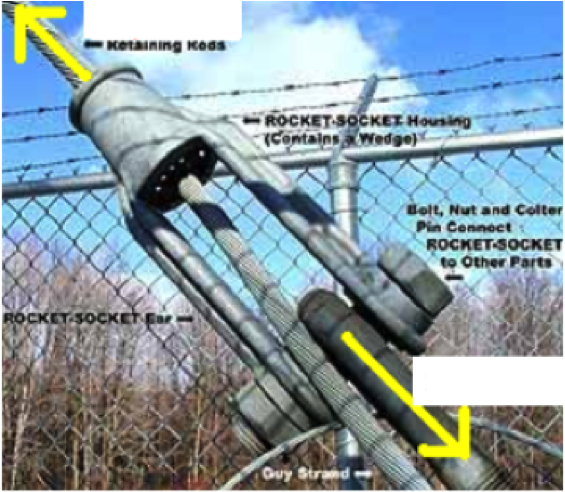
\includegraphics[width=0.5\textwidth]{DESCRIPTION.png}\end{center}

In the analysis part, it is need to find out the points where failure is most possible to happen. In other words, the place where maximum local stress occurs. The design part will be discussed below.

Commercial finite element analysis software suite ANSYS will be used for the entire workflow including 3D modeling, FEM analysis and optimization.
\subsection{Design objectives}
\begin{itemize}
\item The safety factor is required to be at least 2. 
\item The weight of the structure should be minimized.
\item Dimensions should be adjusted in a way that other components (the guy wire and the bolt) will also have a good safefy factor, and the connection between the anchor and other components are safe enough. For example, decrease $D2$ may increase the safety factor and reduce the weight of the anchor itself, but it will reduce the safety factor of the bolt significantly.
\item When possible, avoid hurting people (rounded corners will be preferred); manufacturability will also be considered.
\item Preserve the fundamental shape of original design. The general shape of the frame should be kept consistent with the original design. Redesigning from scratch is therefore not desired. The fixed dimensions should also be respected. 
\end{itemize}

\subsection{Conditions}
The material used to build the cable anchor is structural steel.

Some dimensions are fixed. $H9=25\cm$, $V7=6\cm$, $D1 = 6\cm$.

The cable anchor will be loaded with a axial force of $2\times10^5 N$. On one side, the force will be exerted on the guy wire via a cylindrical surface in a form of frictional force. It can be treated as a fixed support. One the other hand, the force is balanced using a bolt put through two holes. Bearing load can be assumed for the situation.

Symmetrical model can be assumed. 
\section{Program modelling}
\subsection{Geometry}
The top view of original design is shown below:

\begin{center}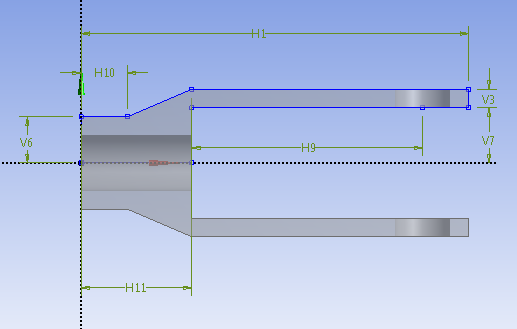
\includegraphics[width=0.75\textwidth]{2D_ORIGIN.png}\end{center}

Where $H1=42\cm$, $H10=5\cm$, $H11=12\cm$, $H9=25\cm$, $V3=2\cm$, $V6=5\cm$, $V7=6\cm$, diameters of all holes are $6\cm$.

It is resembled as below:

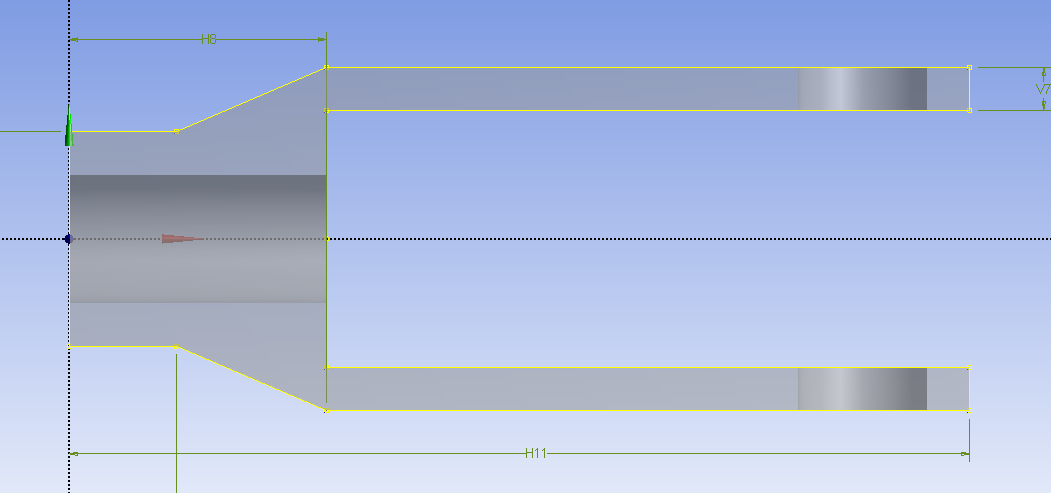
\includegraphics[width=\textwidth]{2D_S_01.PNG}

The 3D model built is then as below, where the height of the component is assumed to be $10 \cm$:

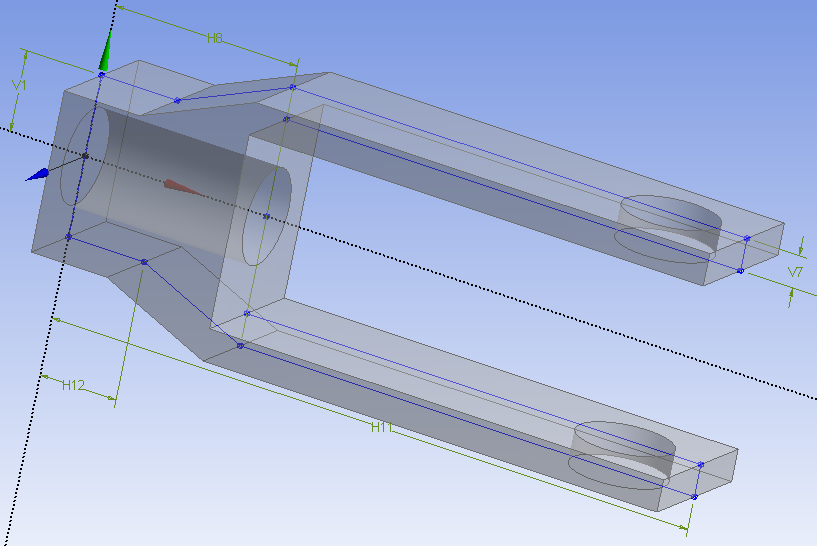
\includegraphics[width=\textwidth]{3D_S_01.PNG}

The dimensions (except the fixed ones), are set as design parameters for the convinience of optimization.
\subsection{Boundary conditions}
The boundary conditions are the loads, where symmetric properties on both axis can be assumed.

On the side of the guy wire, it can be treated as fixed support. One the other side, bearing load can be assumed to be each $1\times10^5 N$, and excerted at the wholes. See the parts below for a fihure demonstrating it.
\subsection{Parameters to optimize}
\subsubsection{Optimization of dimensions only}
In this stage, only the dimensions marked on the provided figure will be optimized. Theshape and topology of the anchor will not be changed. In other words, the optimization will be limited to changing the numbers provided.

To make optimization easier, another set of parameters will be used (note that P6 is not used as the dimension is fixed):

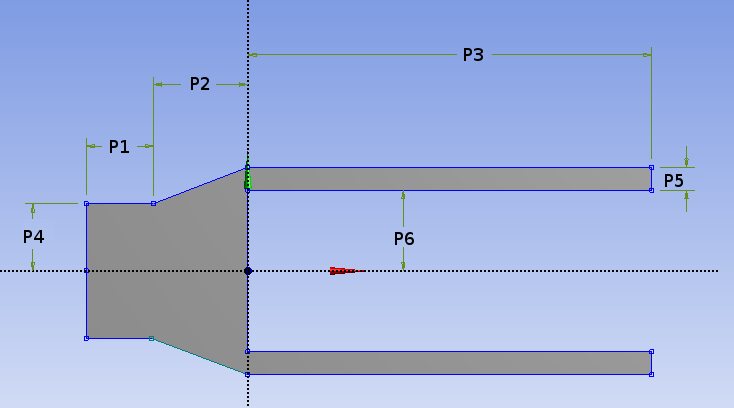
\includegraphics[width=\textwidth]{singleParam/NEW_DIM.PNG}

\begin{align*}
P1 \cm &= H10\\
P2 \cm &= H11-H10\\
P3 \cm &= H1-H11\\
P4 \cm &= V6\\
P5 \cm &= V3\\
P7 \cm &= HEIGHT / 2\\
P8 \cm &= D2
\end{align*}

These parameters will be used in the optimization part of this report.
\subsubsection{Slight shape modification}
In this stage, in addition to dimensional changes, the shape itself will change a little bit.

Some rounded corner (fillets/chamfers) will be added, and an additional extruded structure may be annexed. See the optimization part for details.
\section{FEM analysis}
\subsection{Mesh setup}
As this is a 3D model, elements of tetrahedron shapes are used.

For the mesh, two refinements are added as below, where the first one (\textit{Refinement}) is for the cylindrical surface of loading, and the second one (\textit{Refinement 2}) is for the sharp edges of 90 degree where stress concentration might occur. More refinements will be added in optimization stage to accomodate the changed shape. See the optimization part for details.

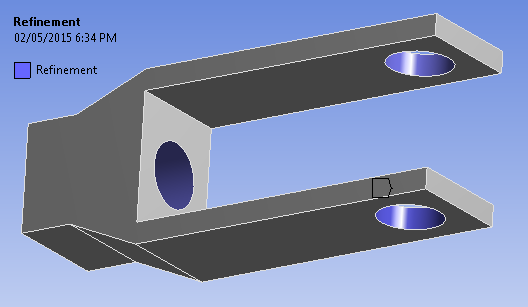
\includegraphics[width=0.5\textwidth]{REF1.PNG}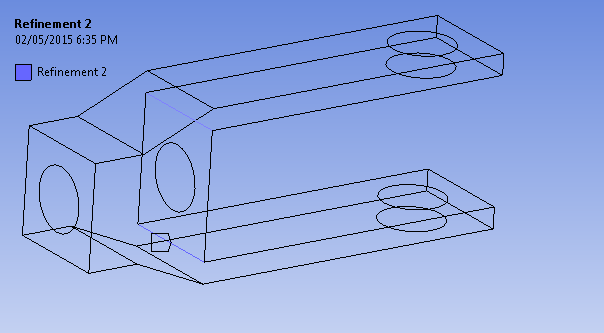
\includegraphics[width=0.5\textwidth]{REF2.PNG}

The overall mesh with a size of $2\cm$ is shown below:

\includegraphics[width=0.5\textwidth]{{MESH_0.02}.PNG}\includegraphics[width=0.5\textwidth]{{MESH_0.02F}.PNG}
\subsection{Boundary conditions setup}
As discussed in previous parts, the load from the guy wire is treated as a fixed support, and the load from the bolt is treated as two bearing loads.

\begin{center}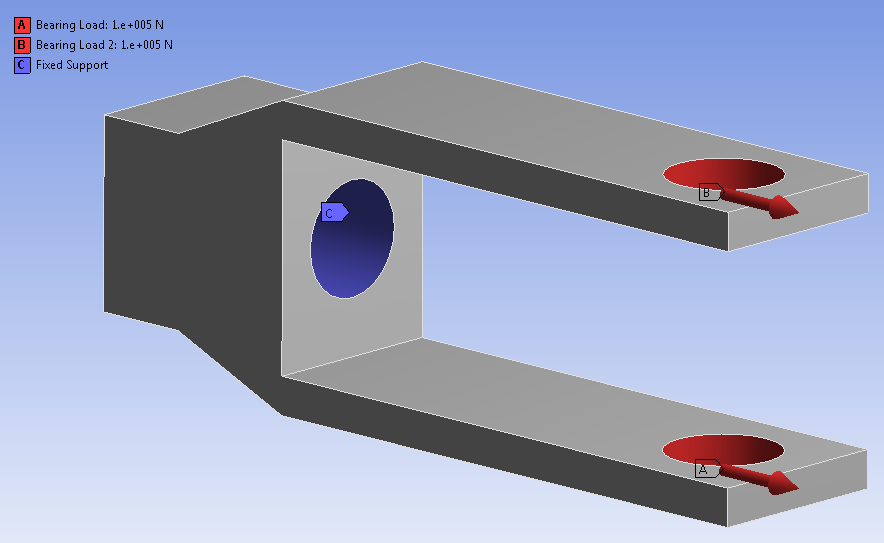
\includegraphics[width=0.75\textwidth]{Model.PNG}\end{center}
\subsection{Results}
The maximum principle stress is found to be around $480\si{\mega\pascal}$.

\begin{center}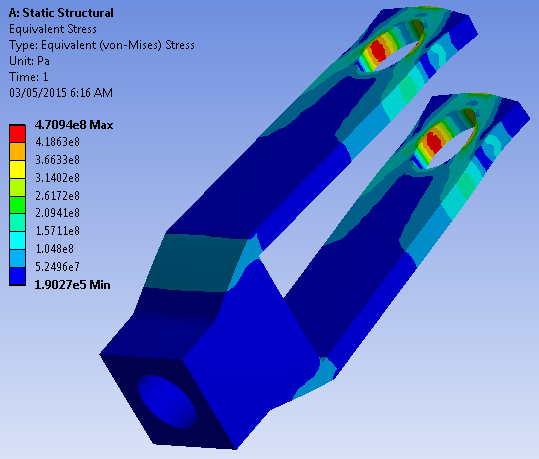
\includegraphics[width=0.75\textwidth]{STRESS_DEFAULT.PNG}\end{center}

As fixed support is assumed on the side of guy wire, and the origin of the coordinate system is also on that side, the maximum displacement is at the right end, around $0.39 \si{\milli\meter}$. Figures can be found in the convergence study part.

We can clear see that the maximum stress is at the four symmetric points: the side end of the wholes. They are exactly the points where failure is most possible to happen.  An enlarged figure below shows it better:

\begin{center}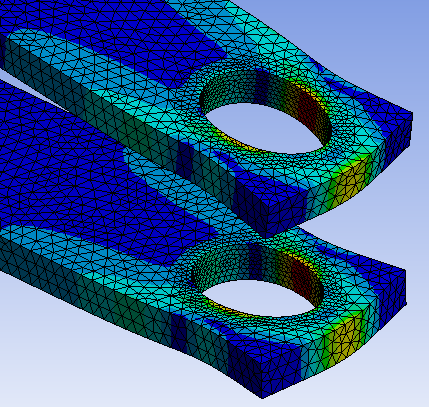
\includegraphics[width=0.5\textwidth]{LOCAL_STRESS.PNG}\end{center}

As uniform material properties is assumed, the local safety factor would be proportional to the local principle stress. The local safety factors are shown below:

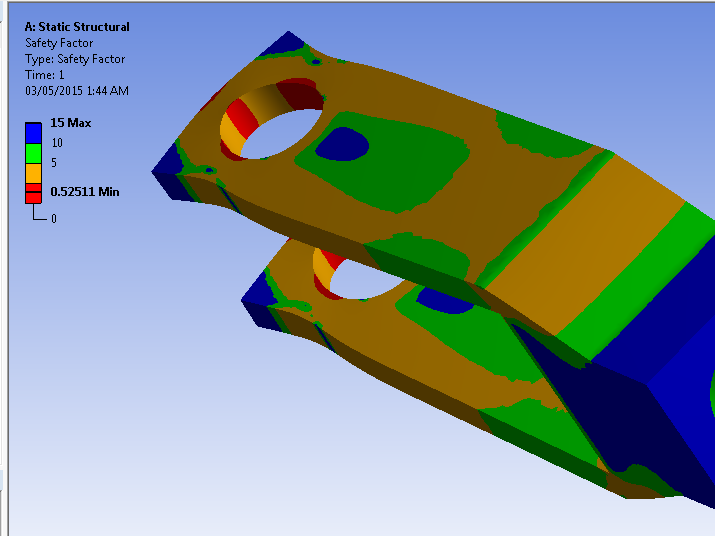
\includegraphics[width=\textwidth]{SF_1.PNG}

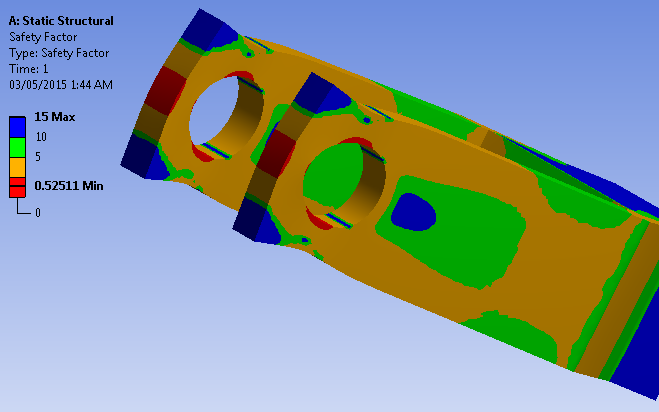
\includegraphics[width=\textwidth]{SF_2.PNG}

Clearly, as the minimum safety factor is around $0.5$, the original design does not meet the requirements.

\subsection{Convergence study}
For convergence study, mesh sizes of  $3\cm$, $2\cm$, $1.5\cm$, $1\cm$, $0.8\cm$ and $0.65\cm$ are used. The mesh of minimum ($0.65\cm$) and maximum ($3\cm$) mesh size are shown below:

\includegraphics[width=0.5\textwidth]{{MESH_0.0065}.PNG}\includegraphics[width=0.5\textwidth]{{MESH_0.03}.PNG}

The results for principle stresses are below, listed in size-decreasing order.

\includegraphics[width=0.5\textwidth]{{STRESS_0.03}.PNG}\includegraphics[width=0.5\textwidth]{{STRESS_0.02}.PNG}
\includegraphics[width=0.5\textwidth]{{STRESS_0.015}.PNG}\includegraphics[width=0.5\textwidth]{{STRESS_0.01}.PNG}
\includegraphics[width=0.5\textwidth]{{STRESS_0.008}.PNG}\includegraphics[width=0.5\textwidth]{{STRESS_0.0065}.PNG}

The results for deformations are below, listed in size-decreasing order.

\includegraphics[width=0.5\textwidth]{{DEFORM_0.03}.PNG}\includegraphics[width=0.5\textwidth]{{DEFORM_0.02}.PNG}
\includegraphics[width=0.5\textwidth]{{DEFORM_0.015}.PNG}\includegraphics[width=0.5\textwidth]{{DEFORM_0.01}.PNG}
\includegraphics[width=0.5\textwidth]{{DEFORM_0.008}.PNG}\includegraphics[width=0.5\textwidth]{{DEFORM_0.0065}.PNG}

The change of both results with mesh sizes can be plotted below (x-axis in reciprocal scale):

\begin{center}
\begin{tikzpicture}[y=20, x=20]
	\tikzstyle{every node}=[font=\footnotesize]

 	%axis
	\draw (0,0) -- coordinate (x axis mid) (20,0);
    	\draw (0,0) -- coordinate (y1 axis mid) (0,10);
    	\draw (20,0) -- coordinate (y2 axis mid) (20,10);
    	
    	%ticks
    	\foreach \x in {0.0065,0.008,0.01,0.015,0.02,0.03}
		\draw ({0.1 / \x},0) -- ({0.1 / \x},0.2)
			node[anchor=south] {\x};
    	\foreach \y in {2,4,...,10}
    		\pgfmathtruncatemacro{\val}{\y *10 + 400}%
		\draw (0,\y) -- (0.2,\y) 
     			node[anchor=west] {\val}; 
    	\foreach \y in {2,4,...,10}
		\pgfmathtruncatemacro{\val}{(\y / 15 + 39) * 100}%
		\draw (20,\y) -- (19.8,\y) 
     			node[anchor=east] {\val}; 
     	
	%labels      
	\node[below=0.5] at (x axis mid) {Mesh size / $\cm$};
	\node[red,rotate=90, above=0.5] at (y1 axis mid) {Max. principle stress / $\si{\mega\pascal}$};
	\node[blue,rotate=-90, above=0.5] at (y2 axis mid) {Max. deformation / $10^{-7}\si{\meter}$};

	%plots
	\draw[red] ({0.1 / 0.03},{(4.2957 - 4) * 10})  --  ({0.1 / 0.02},{(4.5612 - 4) * 10}) -- ({0.1 / 0.015},{(4.7094 - 4) * 10}) -- ({0.1 / 0.011},{(4.75 - 4) * 10}) --  ({0.1 / 0.008},{(4.7325 - 4) * 10}) -- ({0.1 / 0.0065},{(4.7684 - 4) * 10});
	\draw[blue] ({0.1 / 0.03},{(39.225 - 39) * 15}) --  ({0.1 / 0.02},{(39.36 - 39) * 15}) -- ({0.1 / 0.015},{(39.449 - 39) * 15}) -- ({0.1 / 0.011},{(39.485 - 39) * 15}) --  ({0.1 / 0.008},{(39.504 - 39) * 15}) -- ({0.1 / 0.0065},{(39.52 - 39) * 15});
\end{tikzpicture}
\end{center}

We can see it converges. Therefore the results are reasonable and reliable.
\section{Optimization}
The general target of optimization is to achieve a mass (weight) as low as possible, while keeping a safety factor larger than 2.

\subsection{Optimization of dimension only}
\subsubsection{Manual optimization for individual parameters}
Change one parameter at a time, while keeping other parameters the same as original design:
\begin{description}
\item[P1] $=H10$

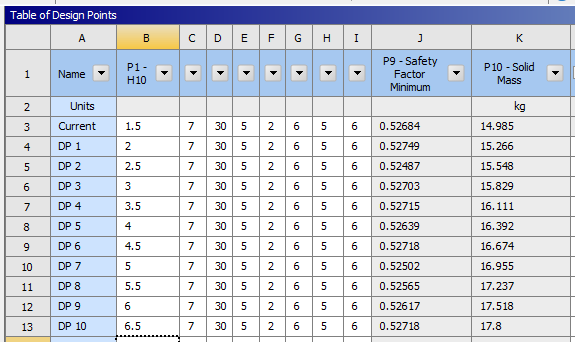
\includegraphics[width=0.75\textwidth]{singleParam/P1.PNG}

It can be seen that $H10$ can be reduced to save weight without decreasing safety factor greatly.
\item[P2] $=H11-H10$

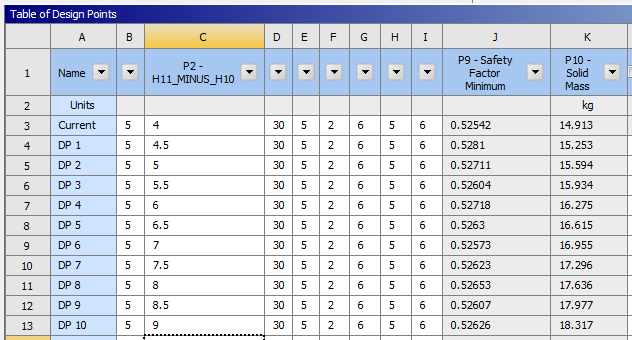
\includegraphics[width=0.75\textwidth]{singleParam/P2.PNG}

It can be seen that $H11$ can be reduced to save weight without decreasing safety factor greatly. Combined with the previous entry, we can seen that $H11$ can be reduced without decreasing safety factor greatly.
\item[P3] $=H1-H11$

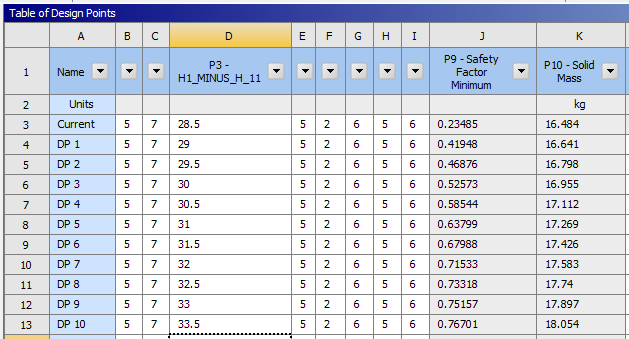
\includegraphics[width=0.75\textwidth]{singleParam/P3.PNG}

It can be seen that reducing $H1 - H11 - H9$, which is the part outer than the bearings, can reduce the safety factor greatly. That value should be increased instead.
\item[P4] $=V6$

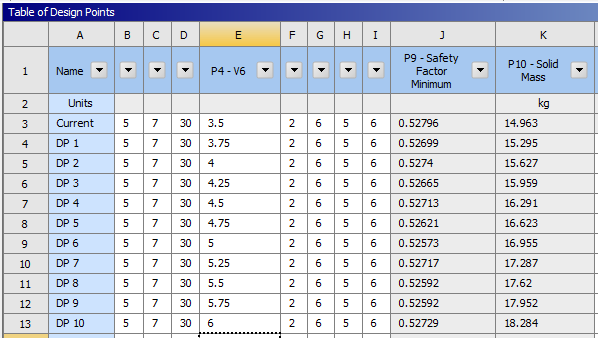
\includegraphics[width=0.75\textwidth]{singleParam/P4.PNG}

It can be seen that $V6$ can be reduced to save weight, and safety factor will not be influenced.
\item[P5] $=V3$

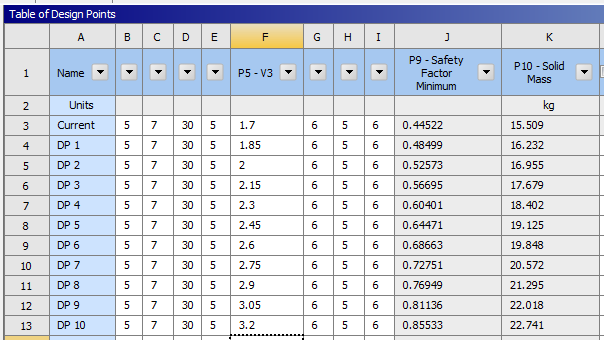
\includegraphics[width=0.75\textwidth]{singleParam/P5.PNG}

It can be seen that increasing $V3$ can increase the safety factor greatly.
\item[P7] $=HEIGHT / 2$

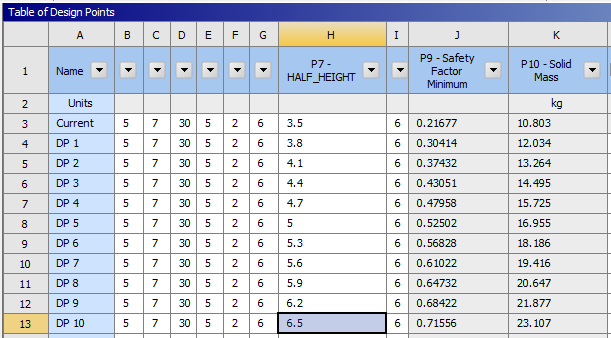
\includegraphics[width=0.75\textwidth]{singleParam/P7.PNG}

It can be seen that increasing the height will increase safety factor greatly. However, the weight will also be increased greatly.
\item[P8] $=D2$

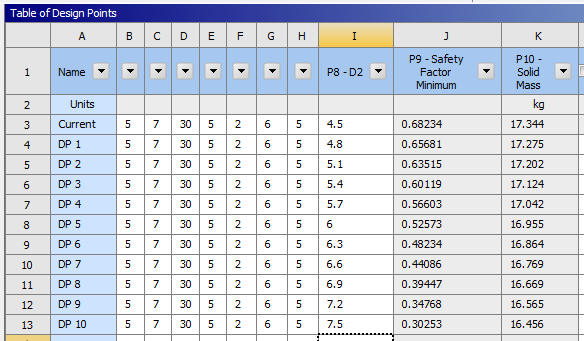
\includegraphics[width=0.75\textwidth]{singleParam/P8.PNG}

It can be seen that reducing $D2$ will increase the safety factor, and reduce the weight slightly. However, as reducing $D2$ will decrease the safety of the bolt significantly, it's preferred that $D2$ is kept at $6\cm$ and not changed.
\end{description}

As P5($V3$) is the most important factor, we focus more on changing $P5$.

According to the result of iteration 1, we try the following values will be used for other parameters:
\begin{align*}
P1 &= 1.5\\
P2 &= 4\\
P3 &= 33.5\\
P4 &= 3.5\\
P7 &= 4.7
\end{align*}

However, this resulted to stress concentration on the cylindrical surface of $D1$. 

\begin{center}
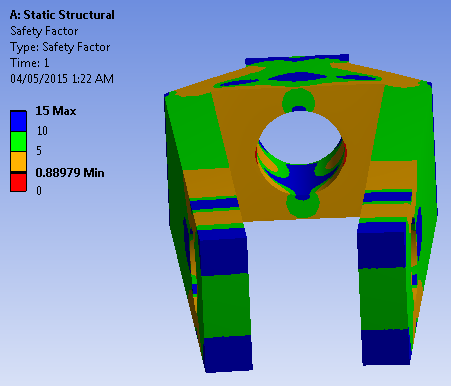
\includegraphics[width=0.5\textwidth]{REF3.PNG}
\end{center}

Therefore, we add mesh refinement to the edge of the hole $D1$ to acquire better results. We found that $P2$ cannot be radically reduced, otherwise the cylindrical surface of $D1$ may fail.

\begin{center}
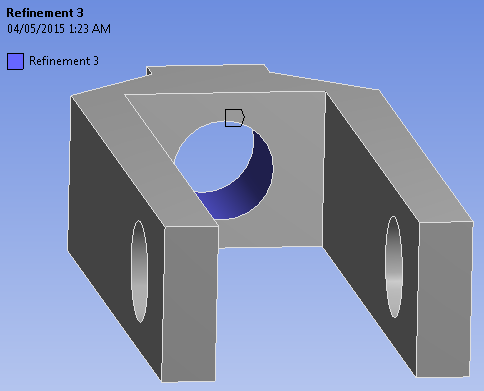
\includegraphics[width=0.75\textwidth]{REF3_SELF.PNG}
\end{center}

As manual optimization is too slow when the number of parameters is large, optimization feature provided by ANSYS is used instead.

\subsubsection{Automatic optimization}
In this stage, ``Direct optimization'' feature is used. The mesh size to be used is $0.8 \cm$, as the license does not permit smaller mesh sizes. 

The targets are set as ``keep safety ratio above 2'' and ``try to minimize the mass''. According to the general idea got in the manual optimization phase, the following settings are used:

\begin{center}
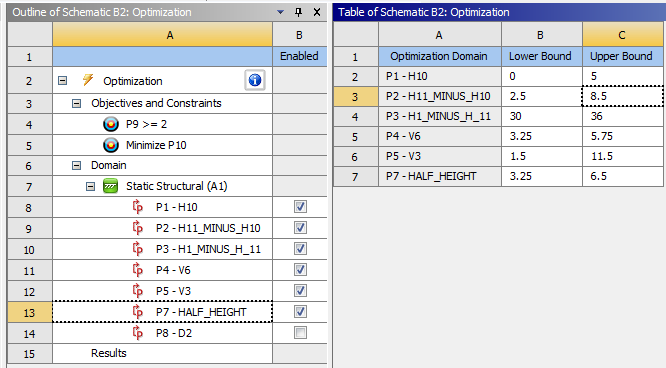
\includegraphics[width=0.75\textwidth]{OPT_BEFORE.PNG}
\end{center}

The following results are acquired:

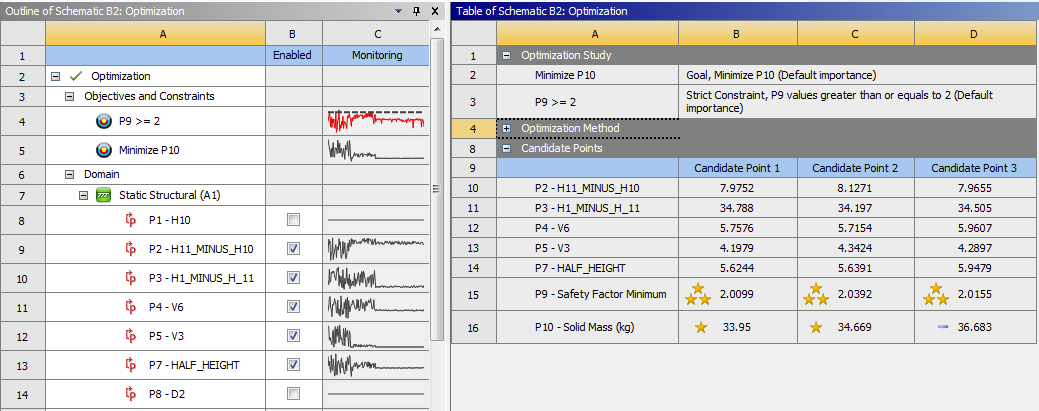
\includegraphics[width=\textwidth]{ASO_RESULT_1.PNG}

Rounding the values, we have the following run:

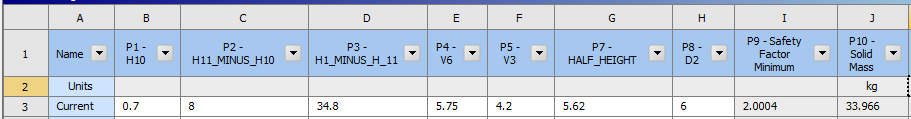
\includegraphics[width=\textwidth]{EX_OPTM_FINAL.PNG}

The optimization workflow yielded a result of:
\begin{align*}
H10 &= P1 \cm = 0.7 \cm\\
H11 &= (P1 + P2) \cm = 8.7 \cm\\
H1 &= H11 + P3 \cm = 8.7 \cm + 34.8 \cm = 43.5 \cm\\
V6 &= P4 \cm = 5.75 \cm\\
V3 &= P5 \cm = 4.2 \cm\\
Height &= P7 * 2 \cm = 11.24 \cm\\
D2 &= 6 \cm 
\end{align*}

In this case, minimum local safety factor is a tiny bit above 2, and the mass of the anchor is $33.97kg$. 

The corresponding model is built below:

\begin{center}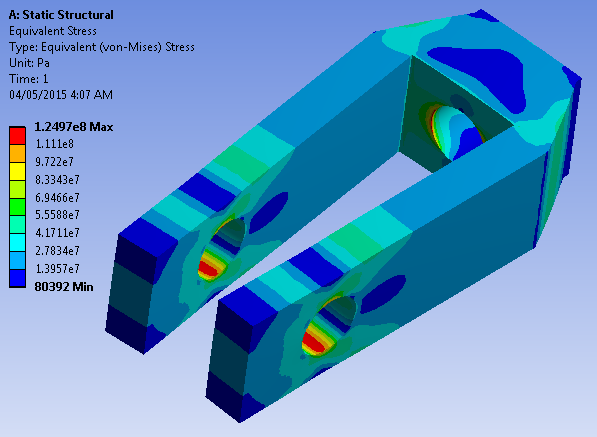
\includegraphics[width=0.75\textwidth]{EX_3.PNG}\end{center}

\begin{center}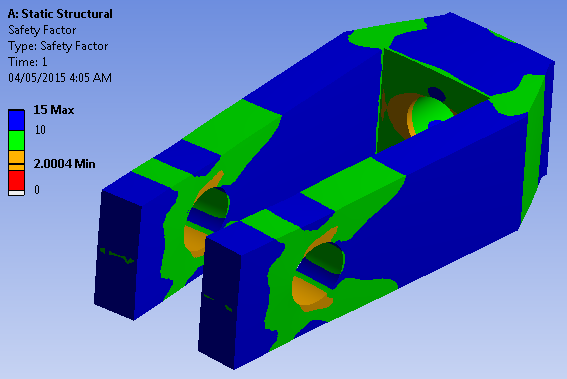
\includegraphics[width=0.75\textwidth]{EX_2.PNG}\end{center}

\begin{center}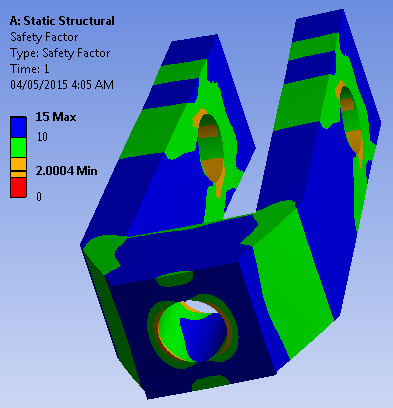
\includegraphics[width=0.5\textwidth]{EX_1.PNG}\end{center}

The mass is verified as

\begin{center}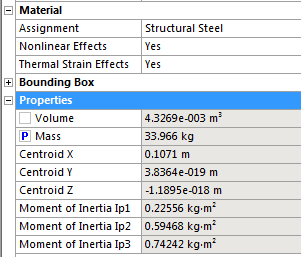
\includegraphics[width=0.5\textwidth]{EX_4.PNG}\end{center}
\subsection{Slight shape modification}
\subsubsection{Shape modifications}
In this stage, two changes are made.

The first change is adding an extruded part at the holes where the bolt will be put. It can increase the area to support the bolt.

The second change is to add rounded corners at all edges. Not only can it reduce the stress concentration, it can also prevent people get hurt by sharp edges.

Additional mesh refinements are needed, as shown below:

\begin{center}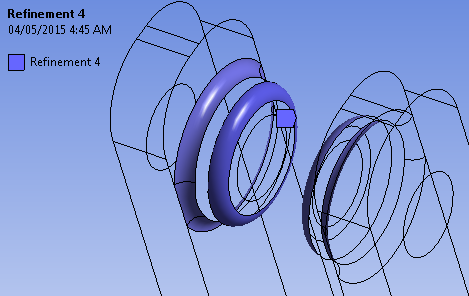
\includegraphics[width=0.75\textwidth]{NX/REF2.PNG}\end{center}

\begin{center}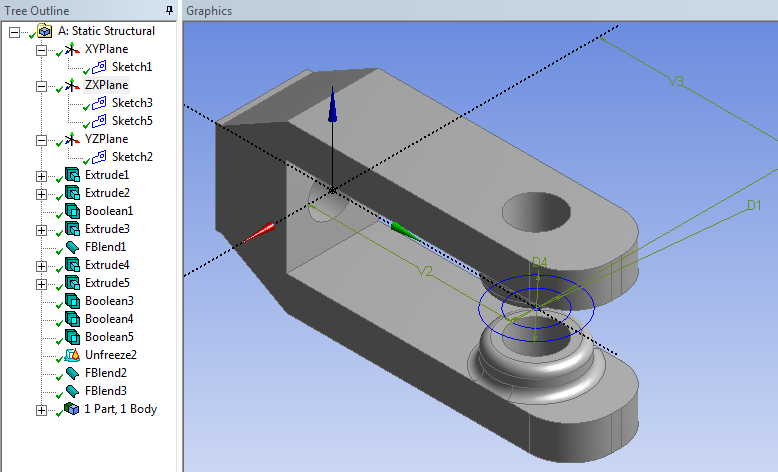
\includegraphics[width=0.75\textwidth]{NX/GEOMETRY.PNG}\end{center}

\begin{center}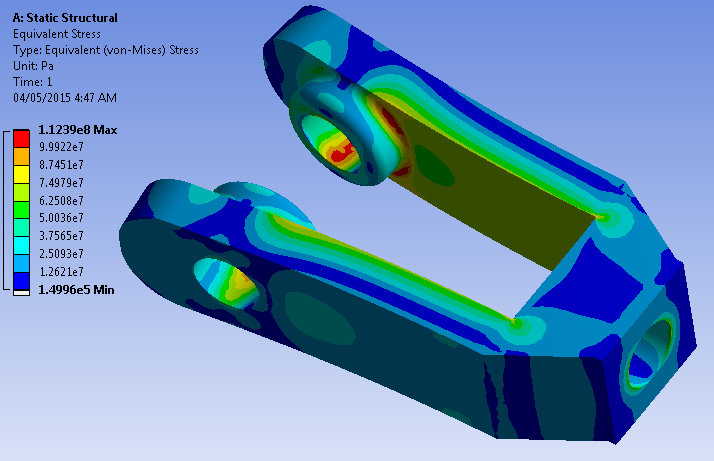
\includegraphics[width=0.75\textwidth]{NX/STRESS.PNG}\end{center}

\begin{center}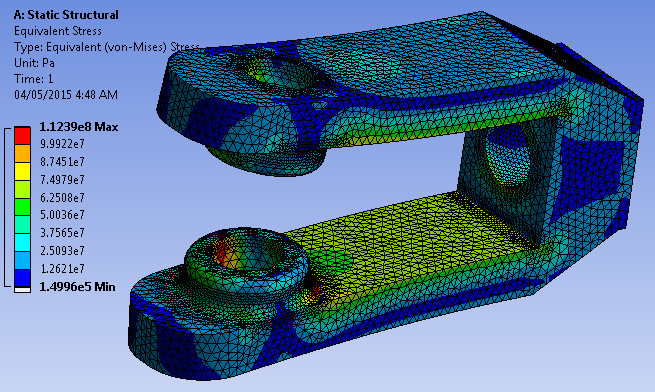
\includegraphics[width=0.75\textwidth]{NX/STRESS2.PNG}\end{center}

From the images, it can be seen that the local principle stress is reduced at the holes for the bolt. Therefore the modification is effective.
\subsubsection{Further dimensional optimization}
Similar to before, the height and the outer radius of the extruded part are set as design parameters. Further optimization process is neccessary to optimize the parameters. As other parameters (e.g. $V3$) can be reduced after the shape modification to save weight, these original parameters also need to be included in the optimization workflow.

/* WORK IN PROGRESS */

The dimensions might not be optimum, as the running optimization flow in ANSYS in the lab is very slow, so only a few samples of design parameters are tested. It would be better if we can rent Tianhe-2 supercomputer to compute.

Further shape modifications are also possible, including using non-uniform crosssesctional area for two arms, using rounded shape at the end for holding the guy wire, and annexing extruded part on the hole for the guy wire, similar to the modifications at the holes for the bolt. Those approaches can reduce weight by using less material using smaller dimensions, while keeping acceptable safety factor by reinforcing the places where local strss is high. Using rounded shape for all parts can reduce the weight and reduce stress concentration at corners. However, those design are not simulated due to time limit. 
\section{Conclusion}
In this design project, the stress of anchor under loading is simulated, and the dimensions and shape of it are optimized using ANSYS finite element analysis tool.

The principles of optimization is discussed. The boundary conditions are set as fixed support and bearing loads. Tetrahedron shaped elements are used to form the mesh, with edges and load points particularly refined. The convergence studies showed that the results are reliable. Notice as the mesh size cannot be further reduced due to ANSYS license limit, the results might not be accurate enough.

We found that the maximum stress is likely to occur at four points, which are the side of the cylindrical surfaces for the bolt. We therefore optimize the design accordingly. Increasing $V3$ worked well for this. $H10$ and $H11$ can be reduced to save weight, yet $H11 - H10$ should not be changed much, otherwise the whole for the guy wire might fail.

In addition to the fixed dimensions in the problem description, $D2$ is not changed either, in order to work well with the bolt safely. In a general target of ``reduce weight as much as possible as long as safety factor stays above 2'', ``direct optimization'' feature provided by ANSYS is used to search for improved parameters.

Modifying the dimension values only, an minimum mass of $33.97$ kg can be achieved while satisfying the safety factor requirement of $2$. 

After adding fillets and annexing an extruded tube to hold the bolt, an minimum mass of $33.97$ kg can be achieved while satisfying the safety factor requirement of $2$. 
\section{Appendix}
The exported ANSYS project files including the simulation results are downloadable below. 
\begin{description}
\item[Original design] \url{https://github.com/kmxz/mech4450project/blob/master/s1.wbpj}.
\item[Optimized design, only dimensions changed] \url{https://github.com/kmxz/mech4450project/blob/master/s2.wbpj}.
\item[Optimized design, with slight shape modification] \url{https://github.com/kmxz/mech4450project/blob/master/s3f.wbpj}.
\end{description}
\end{document}